% This is the aspauthor.tex LaTeX file
% Copyright 2010, Astronomical Society of the Pacific Conference Series

\documentclass[11pt,twoside]{article}
\usepackage{asp2010}

\resetcounters

\bibliographystyle{asp2010}

\markboth{Ceballos, Cobo, Fraga-Encinas, van der Kuur, Schuurmans, Gottardi}{Data Flow design for TES}

\begin{document}

\title{Data Flow design for event detection and qualification 
in TES x-ray detectors}
\author{M.T.~Ceballos$^1$, B.~Cobo$^1$, R.~Fraga-Encinas$^1$, J.~van~der~Kuur$^2$, J.~Schuurmans$^2$, L.~Gottardi$^2$,
\affil{$^1$Instituto de F\'\i sica de Cantabria (CSIC-UC), Avda. de Los Castros s/n, 39005 Santander, Spain}
\affil{$^2$Netherlands Institute for Space Research,Sorbonnelaan 2,3584 CA Utrecht, NL }}

\begin{abstract}
The current and forthcoming research lines in X-ray astronomy will require unprecedented 
spectral resolution with imaging capabilities. The most promising detectors able to provide 
these capabilities are the calorimeters based on Transition Edge Sensor (TES) technologies, like 
the one that has been under development for the proposed ATHENA x-ray space mission.

We present here the Data Flow designed for one of such instruments covering the 
detection algorithms to extract the x-ray events (photons) from the noisy signal (as well as to cope with 
a possible pile-up), the event qualification (event grade) according to the event arrival time
 and proximity to other events, and finally the filtering process applied to these pulses to 
get their energy content, and thus the astronomical source spectrum.

This development is currently part of a collaboration between
IFCA (Spain) and SRON (NL) institutes, as part of a larger project initiated in 2005 and 
named EURECA \citep{deKorte_2009} involving many other institutes in Europe and the USA. This project was created to
design the TES prototype proposed for the XEUS/IXO/ATHENA ESA missions.
\end{abstract}

\section{Introduction}

In the Transition Edge Sensor (TES) devices, the X-ray photons coming from the astronomical sources 
are absorbed by the detector, producing a steep temperature increase and giving rise to current
pulses which are the device response to an abrupt resistance increment in the superconductor element. 
The arrival time, position and energy content of the pulses are then obtained by
analyzing the electrical pulses generated.

As part of this collaboration, we have designed a full suite of software tools \citep{ceballos_2011} 
to detect the pulses generated in this type of devices in response to the incoming X-ray photons 
as well as to characterize the TES instrument. 

The event processing Data Flow presented here (see Fig.~\ref{dataflow}), accounts for the events (photons) 
detection \citep{ceballos_2012} as well as for the events qualification. In addition it implements a calibration mode to
create the library of template pulses that will be finally used to precisely determine the energy content of the high quality pulses.

\begin{figure}
\centering
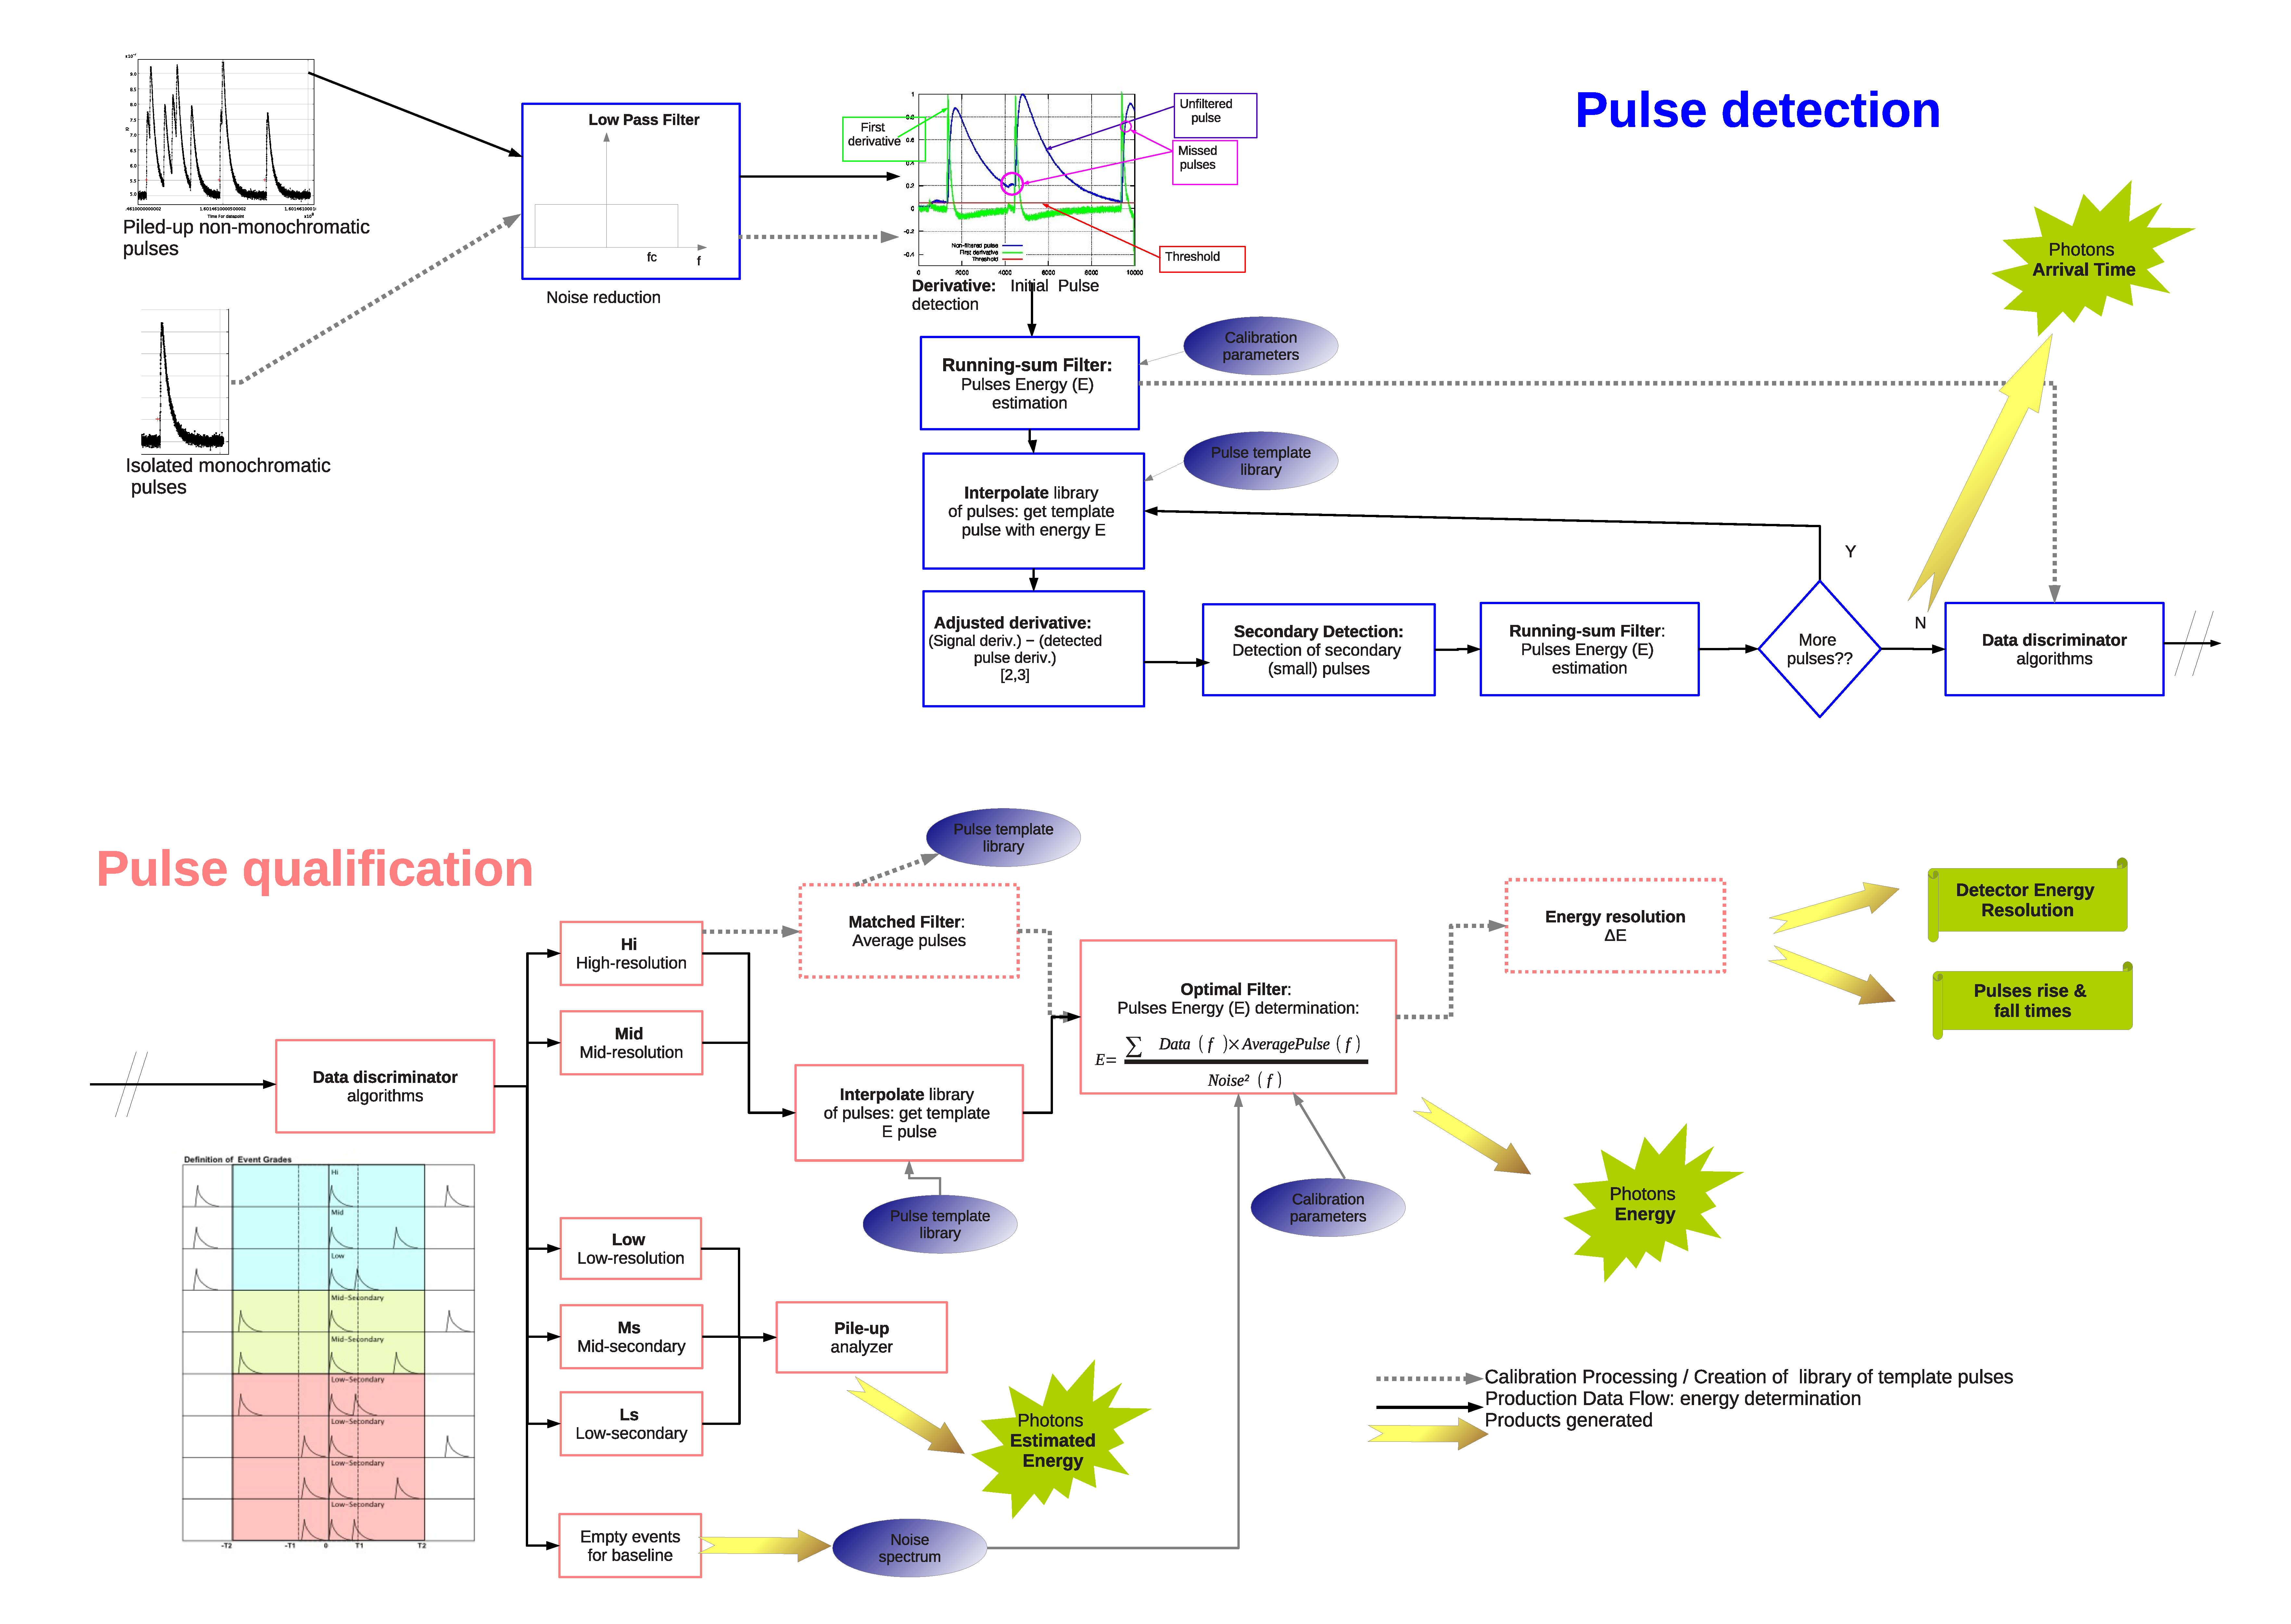
\includegraphics[angle=90,width=1.25\textwidth]{P009_f1.eps} 
\caption{Processing Data Flow: Pulse Detection (in blue boxes) and Pulse Qualification (in salmon boxes)}
\label{dataflow}
\end{figure}

\section{Data Flow I: Event detection}
For the calibration mode, the event detection is done using a set of monochromatic pulses generated by a lab source, while for the 
normal/production processing, the input is a set of \textit{real} source pulses, with different energies and different incoming rates.

The event detection is done through an iterative process with the following steps:

\begin{itemize}
 \item \textbf{Low-pass Filtering}: in order to reduce the noise, the input signal (set of current pulses) is filtered using a low-pass filter
 \item \textbf{First Derivative}: The pronounced peaks in the first derivative of the input signal mark the steep slope of the rising pulse, thus 
 permitting a first detection of the pulses (the small pulses on top of bigger ones are missing in this process if the value of their first
 derivative is not over the initial detection threshold).
 \item \textbf{Running-Sum Filter (RS)} \citep{RS_2011}: this is the sum of $L_{RS}$ digitized data samples, continuously updated upon the arrival 
 of a new data point. Simultaneously, the sum of $L_B$ baseline (no pulses) samples is updated (baseline B filter).
 At the time when $RS/L_{RS}$ reaches its maximum, the pulse height, which is a rough estimator of the pulse energy, can 
 be calculated as 
 
 $ PulseHeight = \frac{RS}{L_{RS}} - \frac{B}{L_B} $
 
 \item \textbf{Interpolation}: Once the energy of the detected pulses is estimated, the template pulses in the calibration library are interpolated to account 
 for these energies.
 \item \textbf{Adjusted derivative} \citep{Boyce_1999}: the first derivative of the detected pulses (using the template pulses) is subtracted from the incoming signal, thus 
 giving prominence to the small pulses previously masked. This is an iterative process, until no further peaks increase the pulse counting.
 The arriving time of the detected photons is saved at this stage. 
 \item \textbf{Data discriminator}: the pulses, with their energy estimation, enters then into the Data Discriminator module to grade their quality. For 
 the \textit{calibration road}, the firstly detected pulses (with their estimated energy) enter directly into the data discriminator to populate the
 calibration library as template pulses if they are qualified as High Quality pulses.
\end{itemize}

\section{Data Flow II: Event Qualification}
\begin{itemize}
 \item \textbf{Grading}: depending on the time between the arrival of successive pulses, these are assigned a grade (High/Mid/Low resolution and Mid/Low
 secondary). Those pulses qualified as High resolution enter the calibration database, if in calibration mode (see above). During production 
 processing these pulses and the Mid quality ones, are selected to get the best possible energy estimation. The low quality and the secondary
 pulses are moved to the pile-up analyzer with the energy previously estimated. The empty events are also used to be incorporated into the calibration 
 database, since they will be used afterwards for the optimal filter creation.
 \item \textbf{Interpolation}: the template pulse in the calibration database are interpolated to get template pulses for the High/Mid quality detected pulses.
 \item \textbf{Optimal Filtering}: the template extracted from the calibration database with the expected shape of the pulse is multiplied with the data, 
 to create a filter. The filter is optimum when it is adjusted based on the noise spectrum. Then, the energy of these pulse can be calculated as:
 
 $ Energy = \sum \frac{Data(f) \times AveragePulse(f)}{Noise^2(f)}$
 
 If in calibration mode, the high quality pulses are also optimally filtered to obtain the energy resolution of the device \citep{ceballos_2012}. 
 In addition the \textit{rise} and \textit{fall} time of the pulses can be studied since they are related to the intrinsic properties of the device.
 
 \item \textbf{Pile-up analyzer}: the piled-up pulses are studied following a process similar to the adjusted derivative one, using the pulse shape 
 information (interpolation in the calibration database).
 \item \textbf{Baseline analyzer}: it is designed to provide the noise spectrum for the optimal filtering and to try to extract the signal bumps too small 
 to be detected during regular pulse triggering.
 
\end{itemize}


\acknowledgements We acknowledge financial support by the Spanish Ministry of Science and Innovation (MICINN) 
under projects ESP2006-13608-C02-01, AYA2009-08059 and AYA2010-21490-C02-01.

\bibliography{P009.bib}

\end{document}
